\documentclass[10pt]{article}
\usepackage[a4paper,margin=1.4cm]{geometry}
\usepackage[T1]{fontenc}
\usepackage{lmodern,microtype,amsmath,booktabs,enumitem,xcolor,tikz}
\usetikzlibrary{arrows.meta,positioning}
\setlist{nosep,leftmargin=1.1em}
\setlength{\parindent}{0pt}
\setlength{\parskip}{3pt}
\pagestyle{empty}
\definecolor{acc}{HTML}{2A6FDB}
\newcommand{\sect}[1]{\par\vspace{4pt}{\color{acc}\bfseries #1}\par\vspace{1pt}}

\begin{document}
{\Large\bfseries privharness: how the privacy harness works}\hfill{\small\texttt{research/privacy-obfuscation/privharness}}\\[2pt]
{\small Input: any labelled video or image dataset with a \emph{task} to keep (e.g.\ the action) and one or more
\emph{secrets} to hide (e.g.\ who is in it, appearance attributes). Output: the obfuscator with the best measured
privacy--utility trade-off, certified by attackers trained on its output.}

\vspace{4pt}
\begin{center}
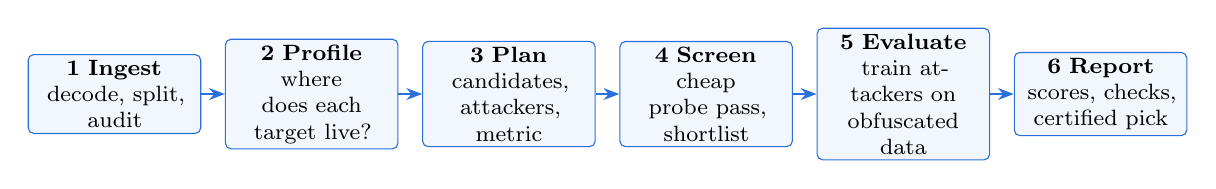
\begin{tikzpicture}[node distance=3mm, every node/.style={font=\footnotesize, align=center},
  box/.style={draw=acc, rounded corners=2pt, fill=acc!6, minimum height=9mm, text width=2.05cm, inner sep=2pt},
  arr/.style={-{Stealth[length=2mm]}, acc, thick}]
\node[box] (i) {\textbf{1 Ingest}\\decode, split,\\audit};
\node[box, right=of i] (p) {\textbf{2 Profile}\\where does each\\target live?};
\node[box, right=of p] (pl) {\textbf{3 Plan}\\candidates,\\attackers, metric};
\node[box, right=of pl] (s) {\textbf{4 Screen}\\cheap probe pass,\\shortlist};
\node[box, right=of s] (e) {\textbf{5 Evaluate}\\train attackers on\\obfuscated data};
\node[box, right=of e] (r) {\textbf{6 Report}\\scores, checks,\\certified pick};
\draw[arr] (i) -- (p); \draw[arr] (p) -- (pl); \draw[arr] (pl) -- (s); \draw[arr] (s) -- (e); \draw[arr] (e) -- (r);
\end{tikzpicture}
\end{center}

\begin{minipage}[t]{0.49\textwidth}
\sect{1. Ingest} (\texttt{ingest.py}, \texttt{adapters/})
\begin{itemize}
\item A JSON description names the media (table or folder + regex), which columns are task, secrets and groups
  (recording, scene, session), and how to split. Media are decoded to uint8 frame arrays at a common size.
\item Splits never put one recording on both sides. The audit flags secret classes missing from a side, tiny
  identity sets, and \textbf{near-duplicate footage across the split} (appearance hash gate, then motion-trace
  correlation $\geq 0.99$; 5/5 planted copies found on KTH, no false alarms).
\end{itemize}

\sect{2. Profile} (\texttt{profile.py}, \texttt{views.py})
\begin{itemize}
\item Each item is turned into \emph{cue views} that keep one kind of information: scene with people blacked out,
  person crop, body keypoints and proportions, posture only, motion, colour, low resolution, and the task label
  alone.
\item A linear probe per (target, view) gives \emph{predictability}: 1.0 = the view tells as much as raw video.
  E.g.\ KTH: action lives in posture (1.0); identity in appearance and scene (0.9).
\end{itemize}

\sect{3. Plan} (\texttt{planner.py}, \texttt{candidates.py})
\begin{itemize}
\item Feasibility: temporal methods need video; stick figures need detectable skeletons.
\item Cue matching: e.g.\ secret in body proportions, task in posture $\Rightarrow$ canonical stick figures first.
\item If the task label alone predicts a secret ($\geq 75\%$), that secret is scored \emph{beyond the task} (conditional metric).
\item Catalogue: blur, downsampling, person removal/blur, motion maps, stick figures, canonical stick figures
  ($\times$1--32), and learned BDQ / BDQ$\to$pool trained against \emph{all} secrets at once.
\end{itemize}

\sect{4. Screen} (\texttt{screen.py})
\begin{itemize}
\item Every fixed candidate obfuscates a sample; frozen-feature probes attack it. The Pareto front and best proxy
  scores form the shortlist. Agreement with full evaluation is reported (rank correlation 0.76--1.00 so far).
\end{itemize}
\end{minipage}\hfill
\begin{minipage}[t]{0.49\textwidth}
\sect{5. Evaluate} (\texttt{evaluate.py}, \texttt{attackers.py}, \texttt{protocols.py})
\begin{itemize}
\item The whole dataset is obfuscated (8-bit, as released). Fresh task models and fresh \textbf{attackers are trained
  on the obfuscated training set} and tested on obfuscated test data: frame CNN, video CNN, skeleton/gait network;
  frozen raw-trained attackers are also run (they understate leakage by a median 17--82 points).
\item Protocols: same split; unseen actions; unseen action + unseen scene; unseen group values.
\end{itemize}

\sect{6. Scores} (\texttt{scoring.py}, \texttt{report.py})
\vspace{-2pt}
{\small\begin{align*}
\text{baseline} &= \max(\text{chance},\ \text{task-label-only attacker})\\
\text{leakage} &= \frac{A_{\text{obf}} - \text{baseline}}{A_{\text{raw}} - \text{baseline}},\qquad
\text{privacy} = 1 - \operatorname{clip}(\text{leakage})\\
\text{utility} &= \frac{u_{\text{obf}} - \text{chance}_u}{u_{\text{raw}} - \text{chance}_u},\qquad
\text{PUS} = \frac{2\,P\,U}{P + U}
\end{align*}}
\vspace{-8pt}
\begin{itemize}
\item $A$ = the \textbf{best} attacker (worst case). 95\% intervals by bootstrapping test recordings.
\item \textbf{Certified} privacy = worst over the pick and its re-runs (2 more seeds, 2$\times$ training, DINOv2 attackers).
\item Checks: raw footage measurably above baseline; all-black video must score at baseline.
\end{itemize}

\sect{Validation (one search per dataset, no hand tuning)}
\vspace{1pt}
{\footnotesize\setlength{\tabcolsep}{4pt}
\begin{tabular}{@{}llrr@{}}
\toprule
dataset & harness pick & utility & privacy$^*$\\
\midrule
KTH (25 people) & canon.\ stick fig.\ $\times$16 & 88.8 & 89.5\\
KTH, new scenario & canon.\ stick fig.\ $\times$16 & 75.5 & 84.8\\
VP-HMDB51 (attributes) & blur people only & 63.3 & 43.4\\
UTD-MHAD (8 people) & 1$\times$2\,px motion map & 53.7 & 51.9\\
Charades (90 homes) & \multicolumn{3}{l}{running}\\
\bottomrule
\end{tabular}}

\begin{itemize}
\item[] {\footnotesize $^*$certified (worst over re-runs), 0--100.}
\item On KTH it independently picked the method found by hand; on UTD-MHAD it overturned a hand-drawn conclusion;
  on VP-HMDB51 its robustness pass caught a stronger attacker.
\end{itemize}

\sect{Run it}
{\footnotesize\texttt{python -m privharness ingest desc.json ROOT}\\\texttt{python -m privharness search ROOT}}\\[2pt]
{\footnotesize Design and references: \texttt{docs/harness.md}. Next: a sealed test set for selection; an LLM that
proposes candidates and attacks, judged by the harness.}
\end{minipage}
\end{document}
